



\section{Context/Problem Statement} \label{sec:context}
This section presents (1) requirements that we aim to 
preserve while refactoring access control policies, and (2) motivation for our proposed approach presented in this paper.

\subsection{Synergy requirement for Access Control Architecture}

Managing access control policies is an one of challenging tasks faced by organizations. 
For example, in policy-based systems, policy authors handle specific 
requirements such as role swap for given temporary assignments, and changes in procedures, 
system resources for protection, users' roles, roles' access rights in an organization.
Moreover, these changes in access control policies should comply with existing business logic in the systems.

\begin{figure}[t]
\begin{center}
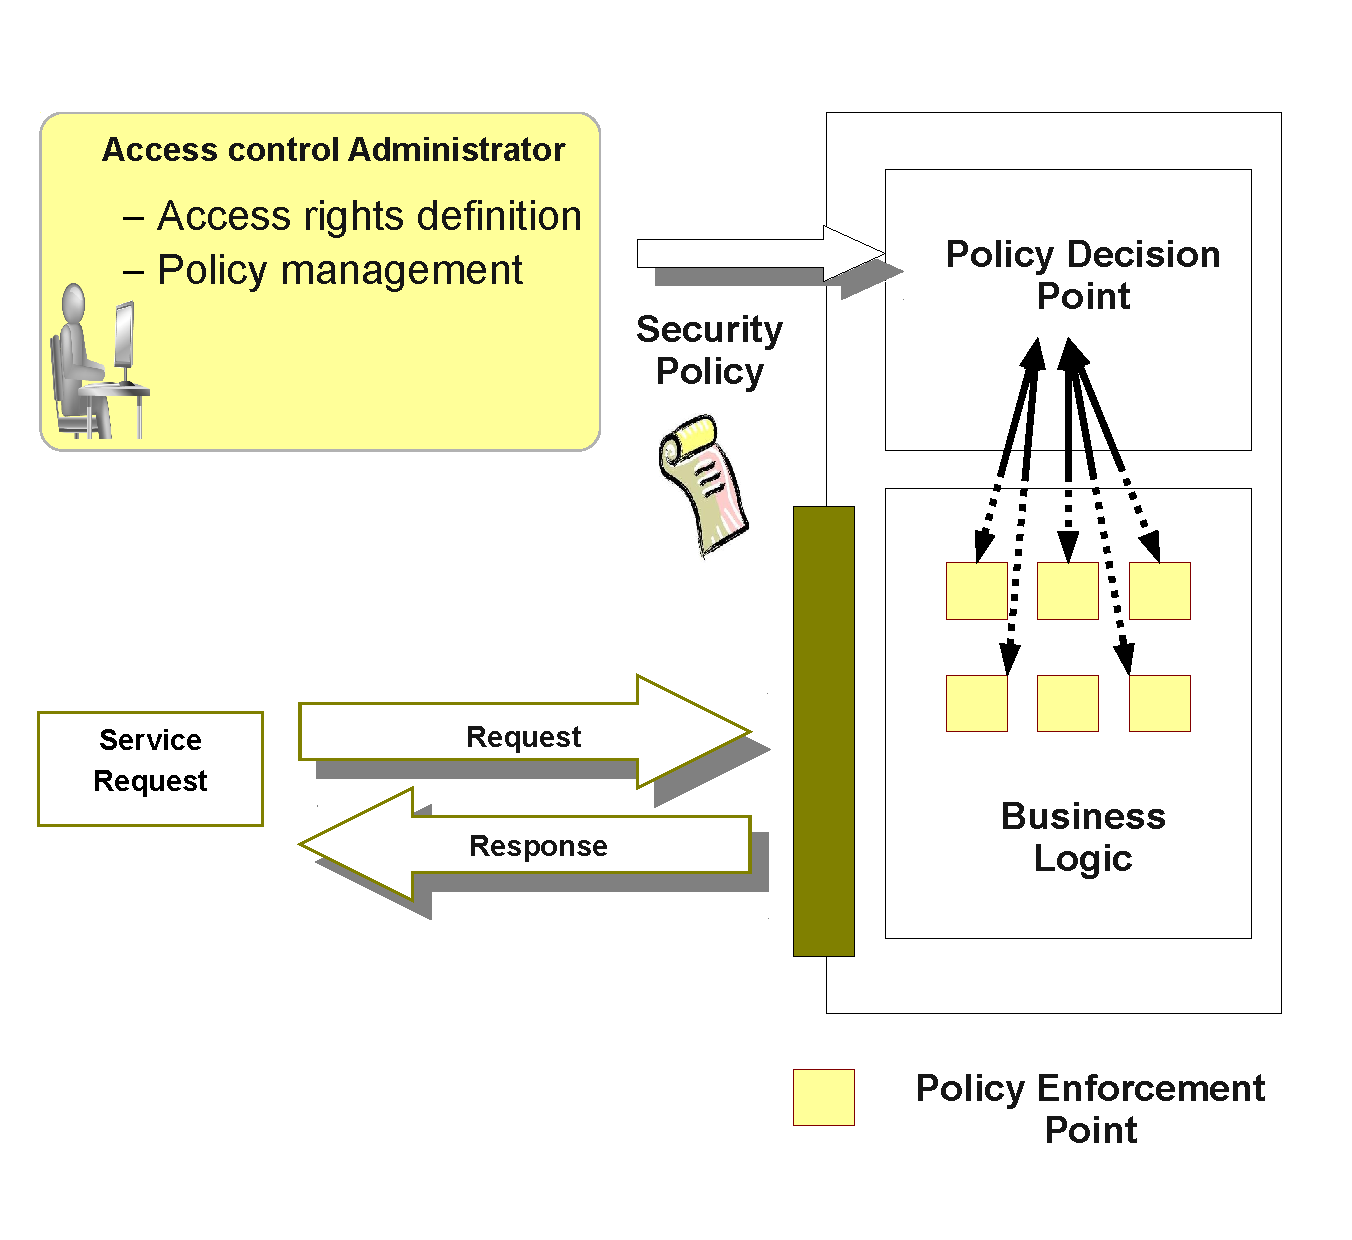
\includegraphics[width=9cm, height=8cm]{business-logic}
\caption{Access Control Request Processing}
\label{pep-pdp}
\end{center}
\end{figure}

To address these issues, there is a great needs for
a simple access control architecture that help handle changes in access control policies easily.
Recently, a popular access control architecture is to handle an access control policy as a separate component 
encapsulated in a PDP. Figure \ref{pep-pdp} illustrates interactions between the PEPs and the PDP: the PEP calls the PDP to 
retrieve an authorization decision based on the encapsulated policy. The PDP evaluates a request against rules in the policy
and return an authorization decision to the PEP.
The separation between the PEP and the PDP in access control systems simplifies policy management across many heterogeneous systems and enables to avoid potential risks arising from incorrect policy implementation, especially when the policy is hardcoded inside the business logic.


 
Along with the reasoning about performance, we maintain the simplicity of the access control architecture based on model 
presented in Figure \ref{model}. In this model, a set of business processes, which comply to users' needs, are encapsulated in a given business logic. The business logic is enforced by multiple PEPs. Conceptually, evaluating request to return an authorization is a decision making process where each PEP interacts with one single PDP. Given an access control request (issued by a given PEP),
the PDP evaluates the request against \emph{only} a single XACML policy and returns its suitable response.
 
\begin{figure}[!h]
\begin{center}
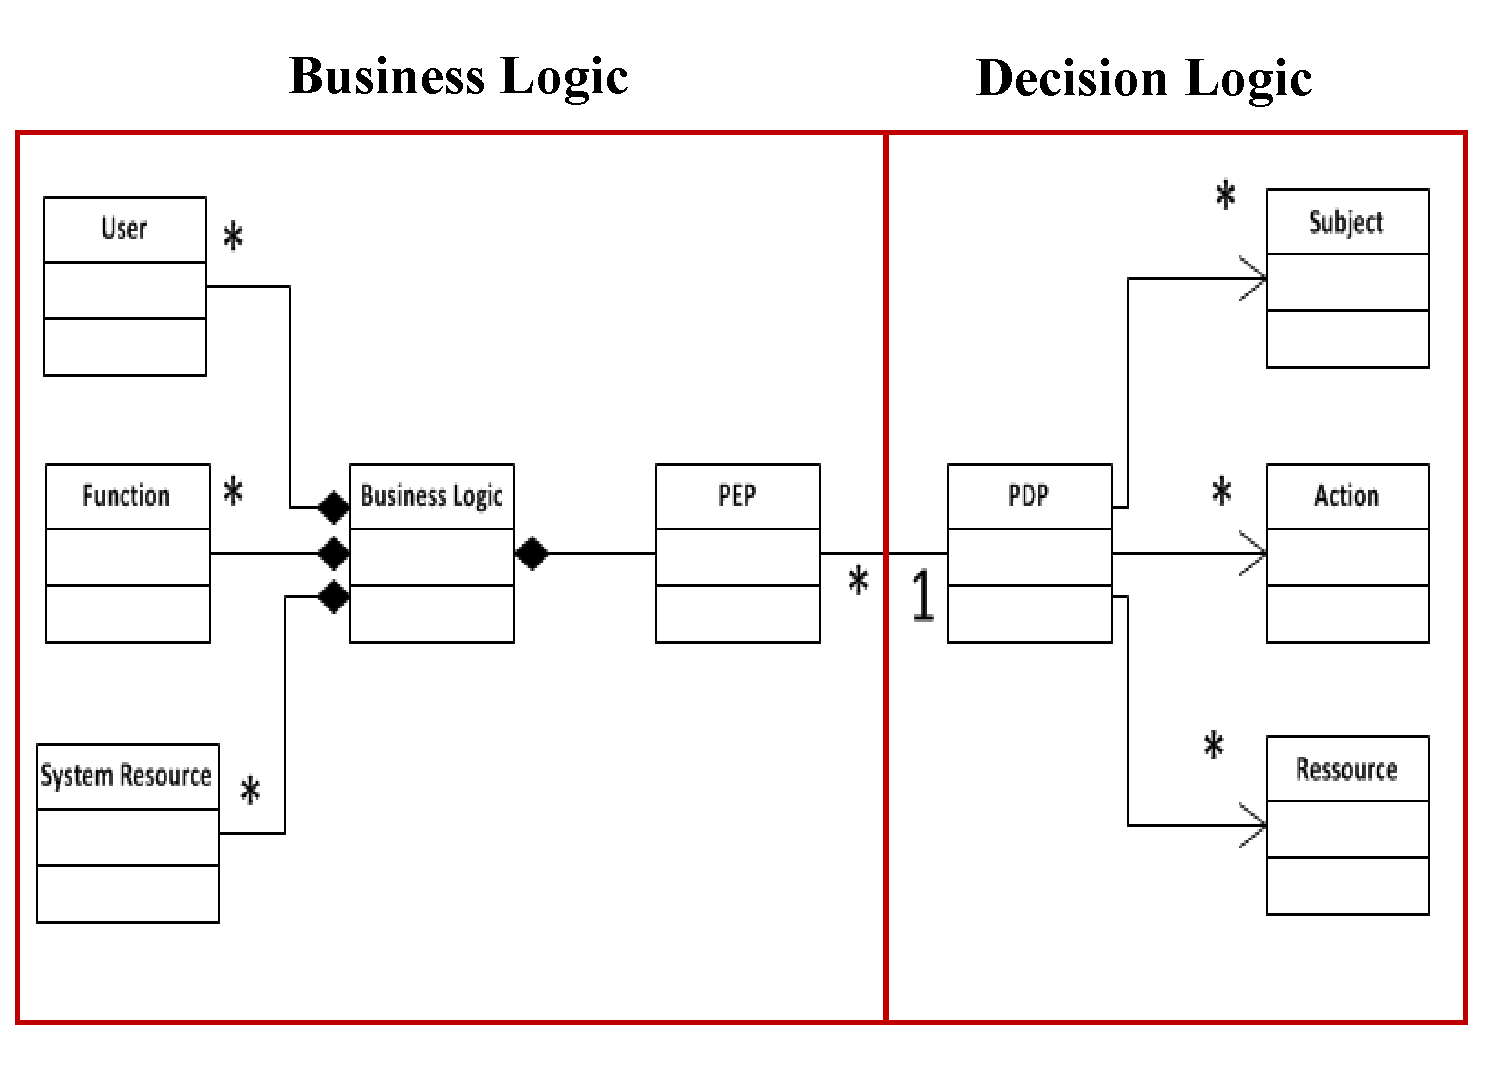
\includegraphics[height=5.5cm,width=8.5cm]{model}
\caption{Access Control Model}
\label{model}
\end{center}
\end{figure}

Given a single policy, administrators are easy to manage a policy and maintain a simple architecture 
where a given PEP is mapped to a fixed single PDP at each decision making process.
Consider that we have multiple policies, each of which is loaded by different PDPs.
In this paper, given multiple PDPs, we define synergy requirement in the access control architecture by mapping a PEPs with a PDP loaded with a suitable access control policy dynamically before deployment. 
The goal behind maintaining synergy requirement helps keep a strong traceability between a policy and the internal 
security mechanisms, which enforces a policy at the business logic level. In such a setting, when administrators update or remove an access control policy, its corresponding PEPs can be easily updated synchronously with the policy changes based on traceability.


%OASIS XACM
%(Organization for the Advancement of Structured Information Standards
%the eXtensible Access Control Modeling Language is an XML-based standard for authorization and access control

\subsection{XACML Access Control Policies and Performance Issues}

In this paper, we focus on access control policies specified in the eXtensible Access Control Modeling Language (XACML)~\cite{sunxacml}.
XACML is an XML-based standard standard policy specification language that defines a syntax of access control policies and
request/response. \\XACML enables administrators to externalize access control policies for the sake of interoperability since access control policies can be designed 
independently from the underlying programming language or platform. Such flexibility enables to easily update access control policies to comply with new requirements.

An XACML is constructed as follows.
A \CodeIn{policy set} element consists of a sequence of \CodeIn{policy elements}, a combining algorithm, and
a \CodeIn{target element}. A \CodeIn{policy element} is expressed through a target, a set of \CodeIn{rules}, and a rule combining algorithm. 
A \CodeIn{target element} consists of the set of resources, subjects, and actions to which a rule is applicable. A \CodeIn{rule} consists of a 
\CodeIn{target element}, a \CodeIn{condition element}, and an \CodeIn{effect}. A \CodeIn{condition element} is a boolean expression that specifies 
environmental context (e.g., time and location restrictions) in which the rule applies.
Finally, an \CodeIn{effect} is rule's authorization decision, which is either permit or deny.

Given a request, a PDP evaluates a request against \CodeIn{rules} in a policy by matching resources, subjects, actions, and condition in the request.
More specifically, an XACML request encapsulates attributes, which define which subject is requested to take an action on which resource in which
condition (e.g., subject Bob is requested to borrow a book).
%This can be under/not a condition.
Given a request, which satisfies \CodeIn{target} and \CodeIn{condition} elements in a rule, the rule's effect
is evaluated as a decision.
If the request does not satisfy \CodeIn{target} and \CodeIn{condition} elements in any rule, its response yields ``NotApplicable'' decision.

When more than one rule is applicable to a request, the combining algorithm helps determine which rule and decision can be finally
applied to the request.
For example, given two rules, which are applicable to the same request and provide different decisions,
the permit-overrides algorithm prioritizes a permit decision over the other decisions.
More precisely, when using the permit-overrides algorithm, the policy evaluation engenders the following three decisions: 

\begin{itemize}
\item Permit if at least one permit rule is applicable for a request.
\item Deny if no permit rule is applicable and at least one deny rule is applicable for a request.
\item NotApplicable if no rule is applicable for a request.
\end{itemize}

Figure \ref{figur1} shows a simplified XACML policy that denies subject Bob to borrow a book in Lines 6-14.

%\fontsize{5}{5}
\begin{figure}[!h]
\begin{center}
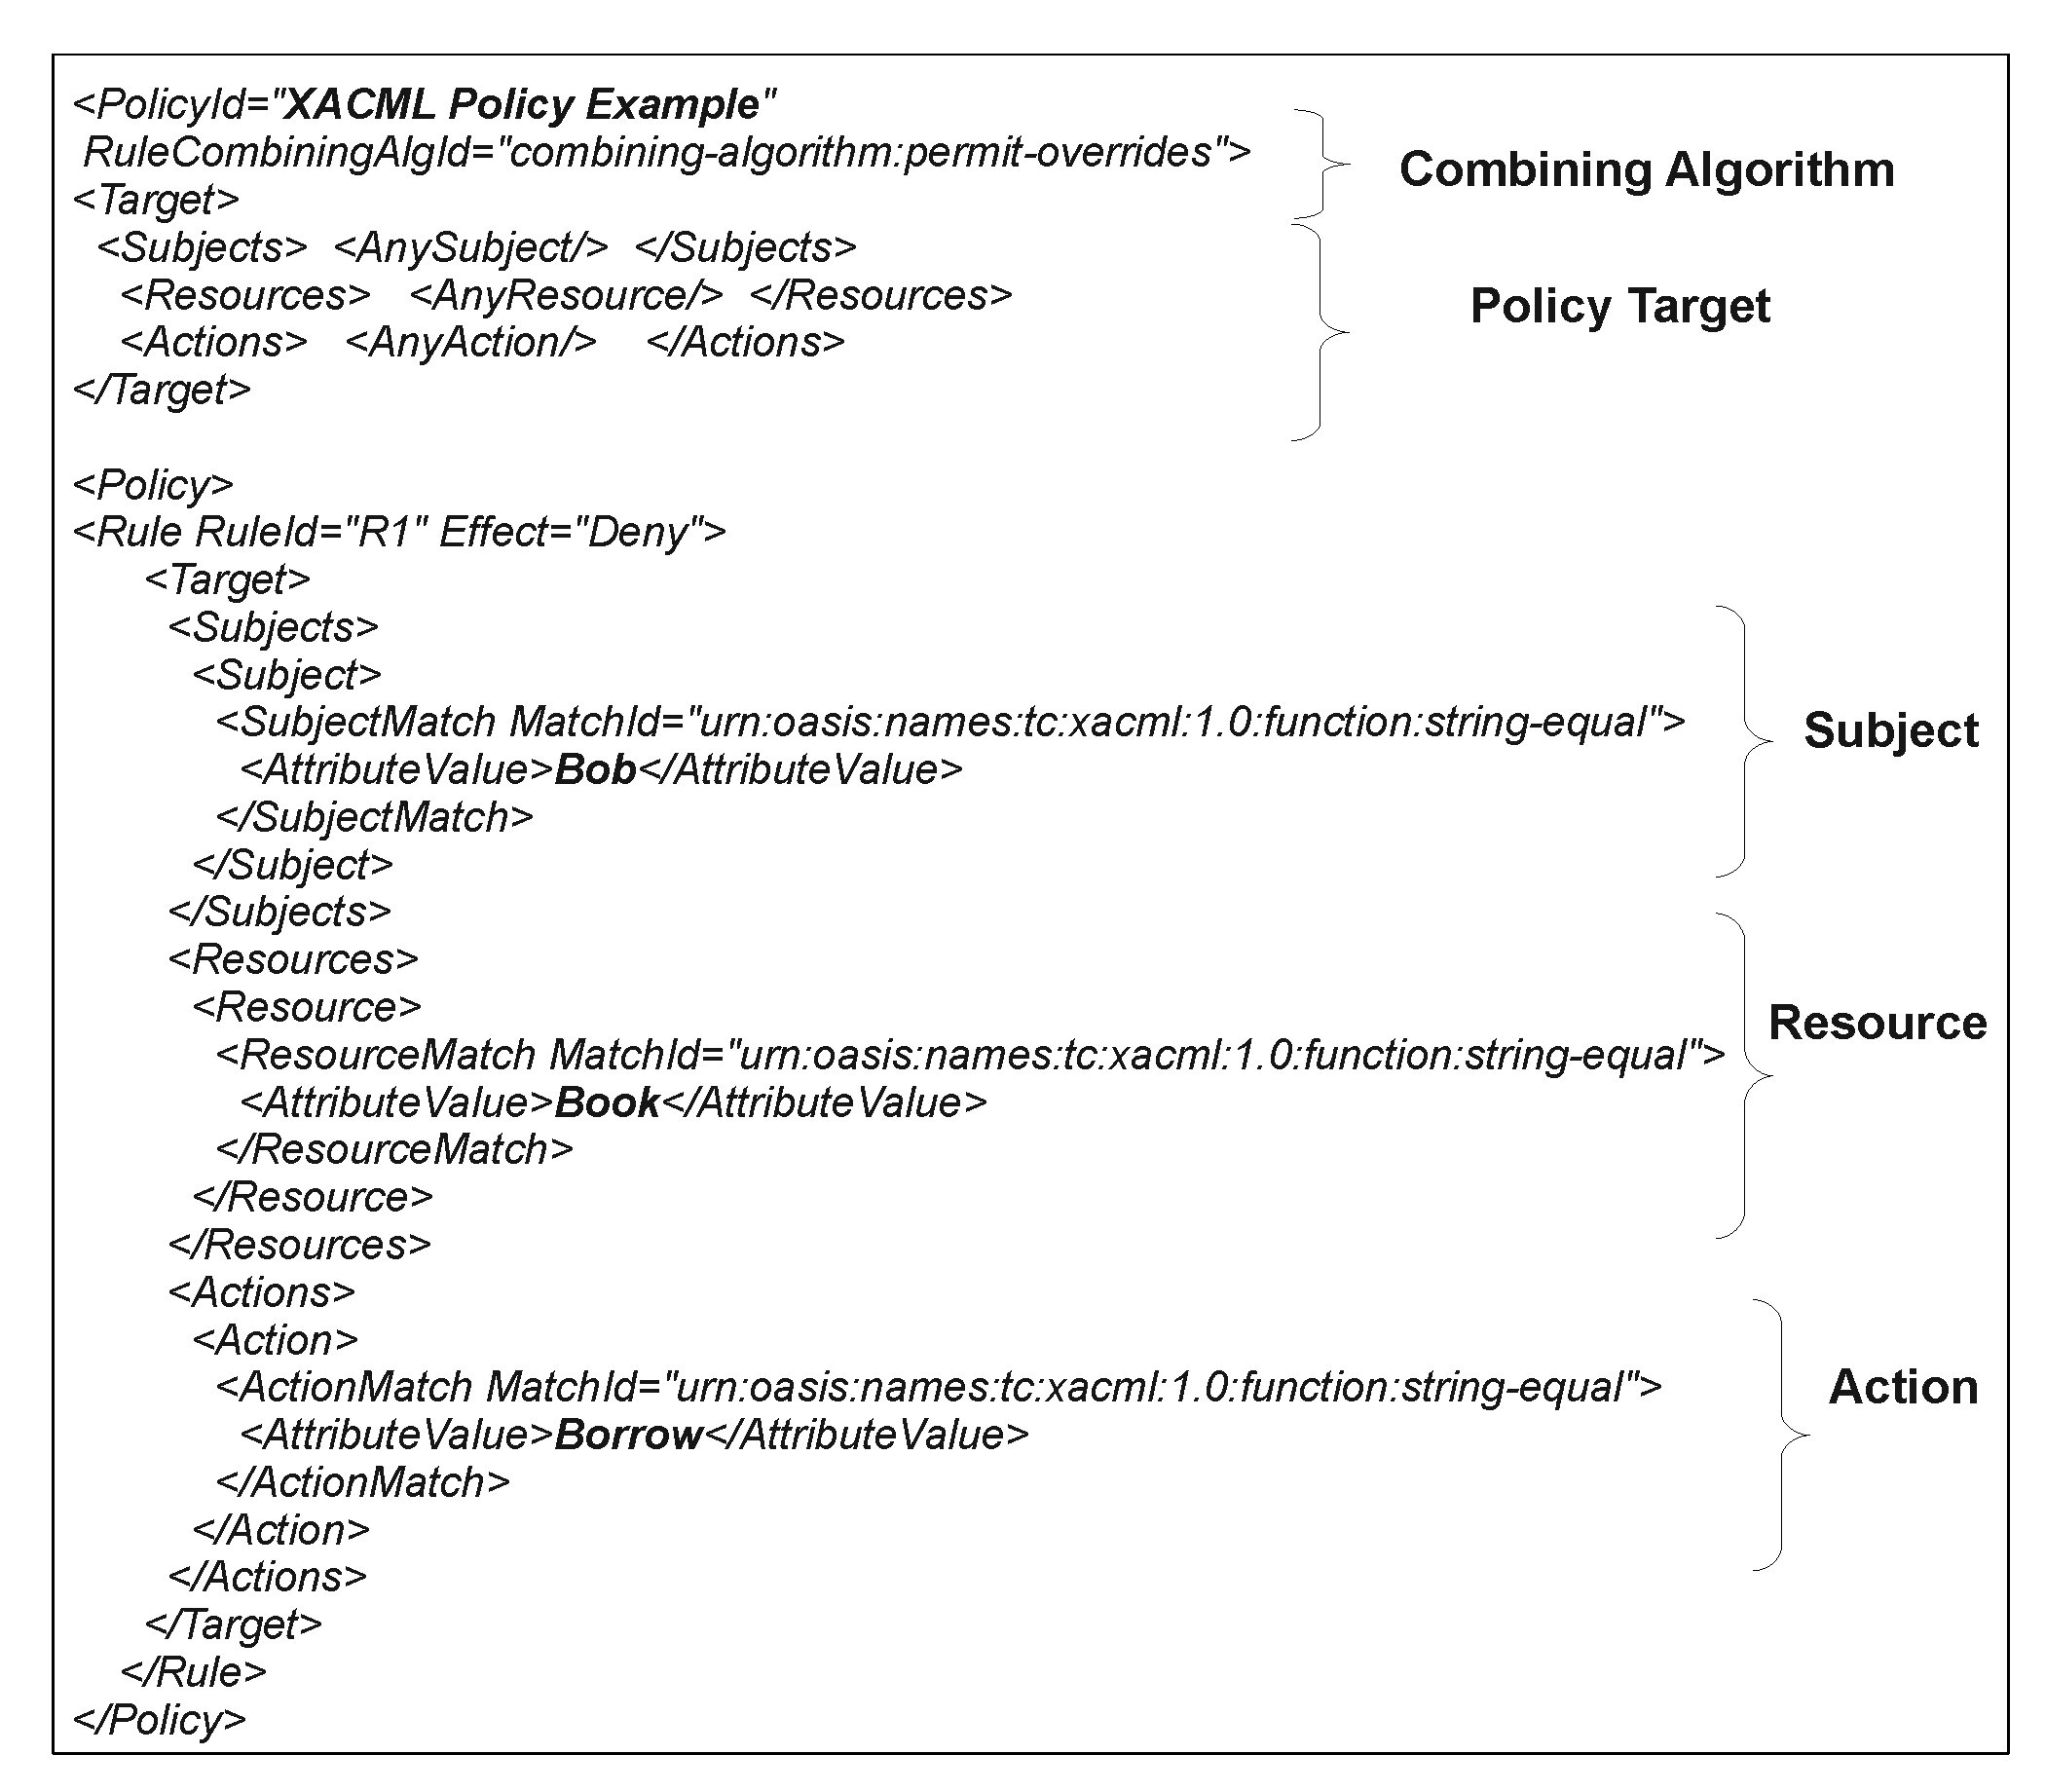
\includegraphics[width=8.6cm]{xacml}
\caption{XACML Policy Example}
\label{figur1}
\end{center}
\end{figure}

 
\Comment{ 
\begin{figure}[!h]%{t}
%\begin{figure}[firstnumber=100]
\begin{CodeOut}
\begin{alltt}
\small
 1 <PolicySet PolicyId="\textbf{An Example Policy Set}" PolicyCombAlgId="\textbf{Permit-overrides}">
 2 <Target/> 
 3  <Policy PolicyId="\textbf{An Example Policy}" RuleCombAlgId="\textbf{Permit-overrides}">
 4   <Target/>
 5    <Rule RuleId="\textbf{1}" Effect="\textbf{Deny}">
 6      <Target>
 7        <Subjects><Subject> \textbf{Bob} </Subject></Subjects>
 8        <Resources><Resource> \textbf{BOOK} </Resource></Resources>
 9        <Actions><Action> \textbf{BORROW} </Action></Actions>
10      </Target>
11	    <Condition>
12        <AttributeValue> \textbf{DEFAULT} </AttributeValue>
13      </Condition>
14    </Rule>
15      <!-- A final, "fall-through" rule that always Denies -->
16    <Rule RuleId="\textbf{FinalRule}" Effect="\textbf{Deny}"/>
17  </policy>
18 </policySet>
\end{alltt}
\end{CodeOut}
\vspace*{-3.0ex} \caption{An XACML Policy Example}
 \label{figur1}
\end{figure}
}
 

%\centering
%\figure[DREF metamodel\label{fig:drefMM}]
%        {\includegraphics[width=0.5\textwidth]{figure/drefMM}}
%\figure[SETER Process: Security Testing for Resilient Systems 
%\label{fig:seter}] {\includegraphics[width=0.49\textwidth]{figure/seter}}
%\caption{DREF and SETER: Conceptual and Operational Frameworks for evaluating resilient systems}
%\end{figure*}


Recently, an XACML policy become more complex to handle increasing complexity of organizations in terms of structure, relationships, activities, and access control requirements. In such a situation, the policy often consists of a large number of rules to specify policy behaviors for various resources, users and actions in the organizations.
In policy-based systems, administrators manage centralized a single PDP loaded with a single policy to govern all of system resources. 
However, due to a large number of rules for evaluation, this centralization raise performance concerns related to request evaluation time for XACML access control policies and may 
degrade the system efficiency and slow down the overall business processes. 

We present following three factors, which may lead to degrade XACML requests evaluation performance: 

\begin{itemize}
\item An XACML policy may contain various attribute elements including \CodeIn{target} elements. Retrieval of
attributes values in the \CodeIn{target} elements for request evaluation may increase the evaluation time.
\item A \CodeIn{policy set} consists of a set of policies. Given a request, a PDP determines final authorization decision (i.e., effect) of the whole \CodeIn{policy set} after combining all of applicable rules' decisions according to the request.
Computation of combining applicable rules' decisions may contribute for a potential evaluation time latency.
\item \CodeIn{Condition} elements in rules can be complex because these elements are built from an arbitrary nesting of non-boolean functions and attributes. In such a situation, evaluating \CodeIn{condition} elements may slow down request evaluation time.
\end{itemize}

